\documentclass[12pt]{article}
\usepackage[left=1cm, right=1cm, top=2cm,bottom=1.5cm]{geometry} 

\usepackage[parfill]{parskip}
\usepackage[utf8]{inputenc}
\usepackage[T2A]{fontenc}
\usepackage[russian]{babel}
\usepackage{enumitem}
\usepackage[normalem]{ulem}
\usepackage{amsfonts, amsmath, amsthm, amssymb, mathtools,xcolor,accents}
\usepackage{blkarray}

\usepackage{tabularx}
\usepackage{hhline}

\usepackage{accents}
\usepackage{fancyhdr}
\pagestyle{fancy}
\renewcommand{\headrulewidth}{1.5pt}
\renewcommand{\footrulewidth}{1pt}

\usepackage{graphicx}
\usepackage[figurename=Рис.]{caption}
\usepackage{subcaption}
\usepackage{float}

%%Наименование папки откуда забирать изображения
\graphicspath{ {./images/} }

%%Изменение формата для ввода доказательства
\renewcommand{\proofname}{$\square$  \nopunct}
\renewcommand\qedsymbol{$\blacksquare$}

%%Изменение отступа на таблицах
\addto\captionsrussian{%
	\renewcommand{\proofname}{$\square$ \nopunct}%
}
%% Римские цифры
\newcommand{\RN}[1]{%
	\textup{\uppercase\expandafter{\romannumeral#1}}%
}

%% Для удобства записи
\newcommand{\MR}{\mathbb{R}}
\newcommand{\MC}{\mathbb{C}}
\newcommand{\MQ}{\mathbb{Q}}
\newcommand{\MN}{\mathbb{N}}
\newcommand{\MZ}{\mathbb{Z}}
\newcommand{\MTB}{\mathbb{T}}
\newcommand{\MTI}{\mathbb{I}}
\newcommand{\MI}{\mathrm{I}}
\newcommand{\MCI}{\mathcal{I}}
\newcommand{\MCR}{\mathcal{R}}
\newcommand{\MJ}{\mathrm{J}}
\newcommand{\MH}{\mathrm{H}}
\newcommand{\MT}{\mathrm{T}}
\newcommand{\MU}{\mathcal{U}}
\newcommand{\MV}{\mathcal{V}}
\newcommand{\MA}{\mathcal{A}}
\newcommand{\MB}{\mathcal{B}}
\newcommand{\MF}{\mathcal{F}}
\newcommand{\ME}{\mathcal{E}}
\newcommand{\MW}{\mathcal{W}}
\newcommand{\ML}{\mathcal{L}}
\newcommand{\MM}{\mathcal{M}}
\newcommand{\MP}{\mathcal{P}}
\newcommand{\VN}{\varnothing}
\newcommand{\VE}{\varepsilon}
\newcommand{\dx}{\, dx}
\newcommand{\dy}{\, dy}
\newcommand{\dz}{\, dz}
\newcommand{\dd}{\, d}


\theoremstyle{definition}
\newtheorem{defn}{Опр:}
\newtheorem{rem}{Rm:}
\newtheorem{prop}{Утв.}
\newtheorem{exrc}{Упр.}
\newtheorem{problem}{Задача}
\newtheorem{lemma}{Лемма}
\newtheorem{theorem}{Теорема}
\newtheorem{corollary}{Следствие}

\newenvironment{cusdefn}[1]
{\renewcommand\thedefn{#1}\defn}
{\enddefn}

\DeclareRobustCommand{\divby}{%
	\mathrel{\text{\vbox{\baselineskip.65ex\lineskiplimit0pt\hbox{.}\hbox{.}\hbox{.}}}}%
}
\DeclareRobustCommand{\ndivby}{\mkern-1mu\not\mathrel{\mkern4.5mu\divby}\mkern1mu}


%Короткий минус
\DeclareMathSymbol{\SMN}{\mathbin}{AMSa}{"39}
%Длинная шапка
\newcommand{\overbar}[1]{\mkern 1.5mu\overline{\mkern-1.5mu#1\mkern-1.5mu}\mkern 1.5mu}
%Функция знака
\DeclareMathOperator{\sgn}{sgn}

%Функция ранга
\DeclareMathOperator{\rk}{\text{rk}}
\DeclareMathOperator{\diam}{\text{diam}}


%Обозначение константы
\DeclareMathOperator{\const}{\text{const}}

\DeclareMathOperator{\codim}{\text{codim}}

\DeclareMathOperator*{\dsum}{\displaystyle\sum}
\newcommand{\ddsum}[2]{\displaystyle\sum\limits_{#1}^{#2}}
\newcommand{\ddssum}[2]{\displaystyle\smashoperator{\sum\limits_{#1}^{#2}}}
\newcommand{\ddlsum}[2]{\displaystyle\smashoperator[l]{\sum\limits_{#1}^{#2}}}
\newcommand{\ddrsum}[2]{\displaystyle\smashoperator[r]{\sum\limits_{#1}^{#2}}}

%Интеграл в большом формате
\DeclareMathOperator{\dint}{\displaystyle\int}
\newcommand{\ddint}[2]{\displaystyle\int\limits_{#1}^{#2}}
\newcommand{\ssum}[1]{\displaystyle \sum\limits_{n=1}^{\infty}{#1}_n}

\newcommand{\smallerrel}[1]{\mathrel{\mathpalette\smallerrelaux{#1}}}
\newcommand{\smallerrelaux}[2]{\raisebox{.1ex}{\scalebox{.75}{$#1#2$}}}

\newcommand{\smallin}{\smallerrel{\in}}
\newcommand{\smallnotin}{\smallerrel{\notin}}

\newcommand*{\medcap}{\mathbin{\scalebox{1.25}{\ensuremath{\cap}}}}%
\newcommand*{\medcup}{\mathbin{\scalebox{1.25}{\ensuremath{\cup}}}}%

\makeatletter
\newcommand{\vast}{\bBigg@{3.5}}
\newcommand{\Vast}{\bBigg@{5}}
\makeatother

%Промежуточное значение для sup\inf, поскольку они имеют разную высоту
\newcommand{\newsup}{\mathop{\smash{\mathrm{sup}}}}
\newcommand{\newinf}{\mathop{\mathrm{inf}\vphantom{\mathrm{sup}}}}

%Скалярное произведение
\newcommand{\inner}[2]{\left\langle #1, #2 \right\rangle }
\newcommand{\linsp}[1]{\left\langle #1 \right\rangle }
\newcommand{\linmer}[2]{\left\langle #1 \vert #2\right\rangle }

%Подпись символов снизу
\newcommand{\ubar}[1]{\underaccent{\bar}{#1}}

%%Шапка для букв сверху
\newcommand{\wte}[1]{\widetilde{#1}}
\newcommand{\wht}[1]{\widehat{#1}}
\newcommand{\ovl}[1]{\overline{#1}}


%%Трансформация Фурье
\newcommand{\fourt}[1]{\mathcal{F}\left(#1\right)}
\newcommand{\ifourt}[1]{\mathcal{F}^{-1}\left(#1\right)}

%%Символ вектора
\newcommand{\vecm}[1]{\overrightarrow{#1\,}}

%%Пространстов матриц
\newcommand{\matsq}[1]{\operatorname{Mat}_{#1}}
\newcommand{\mat}[2]{\operatorname{Mat}_{#1, #2}}

%Оператор для действ и мнимых чисел
\DeclareMathOperator{\IM}{\operatorname{Im}}
\DeclareMathOperator{\RE}{\operatorname{Re}}
\DeclareMathOperator{\li}{\operatorname{li}}
\DeclareMathOperator{\GL}{\operatorname{GL}}
\DeclareMathOperator{\SL}{\operatorname{SL}}
\DeclareMathOperator{\Char}{\operatorname{char}}
\DeclareMathOperator\Arg{Arg}
\DeclareMathOperator\ord{ord}

%Оператор для образа
\DeclareMathOperator{\Ima}{Im}

%Делимость чисел
\newcommand{\modn}[3]{#1 \equiv #2 \; (\bmod \; #3)}
\newcommand{\nmodn}[3]{#1 \not\equiv #2 \; (\bmod \; #3)}

%%Взятие в скобки, модули и норму
\newcommand{\parfit}[1]{\left( #1 \right)}
\newcommand{\modfit}[1]{\left| #1 \right|}
\newcommand{\sqparfit}[1]{\left\{ #1 \right\}}
\newcommand{\normfit}[1]{\left\| #1 \right\|}

%%Функция для обозначения равномерной сходимости по множеству
\newcommand{\uconv}[1]{\overset{#1}{\rightrightarrows}}
\newcommand{\uconvm}[2]{\overset{#1}{\underset{#2}{\rightrightarrows}}}

%% Функция для добавления круга сверху множества
\newcommand{\Circ}[1]{\accentset{\circ}{#1}}

%%Функция для обозначения нижнего и верхнего интегралов
\def\upint{\mathchoice%
	{\mkern13mu\overline{\vphantom{\intop}\mkern7mu}\mkern-20mu}%
	{\mkern7mu\overline{\vphantom{\intop}\mkern7mu}\mkern-14mu}%
	{\mkern7mu\overline{\vphantom{\intop}\mkern7mu}\mkern-14mu}%
	{\mkern7mu\overline{\vphantom{\intop}\mkern7mu}\mkern-14mu}%
	\int}
\def\lowint{\mkern3mu\underline{\vphantom{\intop}\mkern7mu}\mkern-10mu\int}

%%След матрицы
\DeclareMathOperator*{\tr}{tr}

\DeclareMathOperator*{\symdif}{\bigtriangleup}

% Верхние\нижние пределы
\DeclareMathOperator*\lowlim{\underline{lim}}
\DeclareMathOperator*\uplim{\overline{lim}}

\makeatletter
\renewcommand*\env@matrix[1][*\c@MaxMatrixCols c]{%
	\hskip -\arraycolsep
	\let\@ifnextchar\new@ifnextchar
	\array{#1}}
\makeatother


%% Переопределение функции хи, чтобы выглядела более приятно
\makeatletter
\@ifdefinable\@latex@chi{\let\@latex@chi\chi}
\renewcommand*\chi{{\@latex@chi\smash[t]{\mathstrut}}} % want only bottom half of \mathstrut
\makeatletter

\setcounter{MaxMatrixCols}{20}


\begin{document}
\lhead{Действительный анализ}
\chead{Дьяченко М.И.}
\rhead{Лекция - 7}

\section*{Сходимость по мере и её свойства}
В теории вероятности эта  сходимость ещё называется сходимостью по вероятности. Пусть у нас есть измеримое пространство $(X,\MM,\mu)$.

\begin{defn}
	Пусть последовательность $\{f_n(x)\}_{n = 1}^{\infty}$ и $f(x)$ измеримы и конечны на $X$. Тогда говорят, что $f_n(x)$ \uwave{сходится по мере} на $X$ к $f(x)$ в том и только в том случае, когда:
	$$
		\forall \VE > 0, \, \lim\limits_{n \to \infty}\mu(\{x \in X \colon |f_n(x) - f(x)| > \VE\}) = 0
	$$
	Или подробнее:
	$$
		\forall \VE > 0, \, \gamma > 0, \, \exists \, N \colon \forall n \geq N, \, \mu(\{x \in X \colon |f_n(x) - f(x)| > \VE\}) < \gamma
	$$
	\textbf{\uline{Обозначение}}: $f_n \xRightarrow{\mu}f$ или $f_n \xRightarrow{\mu, X} f$.
\end{defn}

\begin{theorem}
	Пусть $(X,\MM,\mu)$ - конечное ИП (то есть $\mu(X) < \infty$), $\{f_n(x)\}_{n =1 }^{\infty}$, $f(x)$ - измеримы и конечны на $(X,\MM, \mu)$. Пусть также открытое $G \subseteq \MR^1$, $g(t) \in C(G)$ (непрерывная на $G$) и верно:
	$$
		\forall n, \, f_n  \colon X \to G, \, f \colon X \to G, \, f_n \xRightarrow{\mu}f 
	$$
	Тогда: $g(f_n) \xRightarrow{\mu} g(f)$.
\end{theorem}
\begin{proof}
	Согласно теореме $4$ лекции $5$ открытое множество можно представить в виде: $G = \bigsqcup\limits_{n = 1}^{\infty}(\alpha_n,\beta_n)$, следовательно существует последовательность компактов:
	$$
		K_1 \subset K_2 \subset \dotsc \subset K_n \subset \dotsc \subset G \colon G = \bigcup\limits_{n = 1}^{\infty} K_n
	$$
	поскольку каждый интервал можно приблизить компактами и приближая $n$-ым компактом первые $n$ интервалов мы, увеличивая количество интервалов, приблизим всё $G$. Рассмотрим прообразы: 
	$$
		f^{-1}(K_n) \equiv E_n, \, n = 1,2, \dotsc \Rightarrow E_1 \subseteq E_2 \subseteq \dotsc \subseteq E_n \subseteq \dotsc, \,  X = \bigcup\limits_{n = 1}^{\infty} E_n
	$$
	поскольку $G$ исчерпывается компактами и $f$ отображает весь $X$ в $G$. Так как $\mu(X) < \infty$, то по утверждению о непрерывности меры (смотри утверждение $2$, лекция $4$) будет верно:
	$$
		\mu(X \setminus E_n) \xrightarrow[n \to \infty]{} 0
	$$
	Пусть заданы произвольные $\VE > 0$ и $\gamma > 0$, выберем $n_0$ такое, что $\mu(X \setminus E_{n_0}) < \tfrac{\gamma}{2}$. Рассмотрим расстояние:
	$$
		d = \rho(K_{n_0}, \MR^1 \setminus G) = \inf\limits_{\substack{x \in K_{n_0} \\ y \in \MR^1 \setminus G} }|x - y| = \min\limits_{\substack{x \in K_{n_0} \\ y \in \MR^1 \setminus G} }|x - y| > 0
	$$
	где для любого фиксированного $x$ расстояние до замкнутого множества достигается: поскольку мы рассматриваем непрерывную функцию на компакте, равную расстоянию до $\MR^1 \setminus G$ и следовательно на компакте она достигает своего минимума, а расстояние больше нуля, поскольку множества не пересекаются ($K_{n_0}$ содержится внутри $G$). Введём множество:
	$$
		K' = \{y \in \MR^1 \colon \rho(K_{n_0}, y) \leq \tfrac{d}{2} \}
	$$
	оно замкнуто, а поскольку $K_{n_0}$ было ограниченным множеством и мы отходим от него не дальше, чем на $\tfrac{d}{2}$, то $K'$ ещё и ограничено $\Rightarrow K'$ это компакт. Кроме того, $K' \subset G$. По условию $g(t) \in C(G)$, то есть непрерывна на $G$, тогда $g(t)$ непрерывна на компакте $K'$. В результате:
	$$
		\exists\, \delta > 0 \colon \forall z,y \in K', \, |z - y| \leq \delta \Rightarrow |g(z) - g(y)| < \VE
	$$
	По условию сходимости по мере:
	$$
		\exists \, N \colon \forall n \geq N, \, A_n = \{x \in X \colon |f_n(x) - f(x)| > \min(\tfrac{d}{2}, \delta)\} \Rightarrow \mu(A_n) < \dfrac{\gamma}{2}
	$$
	Предположим, что $n \geq N$ и $x \not\in A_n \cup (X \setminus E_{n_0})$, тогда:
	\begin{enumerate}[label=\arabic*)]
		\item $f(x) \in K_{n_0} \subseteq K'$, поскольку так мы выбирали $E_{n_0}$ и $K_{n_0} \subseteq K'$ по построению $K'$;
		\item $|f_n(x) - f(x)| \leq \tfrac{d}{2}$, вместе с первым свойством из этого следует, что: $f_n(x) \in K'$;
		\item $|f_n(x) - f(x)| \leq \delta$, вместе со вторым свойством из этого следует, что: $|g(f_n)(x) - g(f)(x)| < \VE$;
	\end{enumerate}
	Следовательно, $F_{n,\VE} = \{x \in X \colon |g(f_n)(x) - g(f)(x)| > \VE\} \subset A_n \cup (X \setminus E_{n_0})$, тогда:
	$$
		\mu(F_{n,\VE}) \leq \mu(A_n) + \mu(X \setminus E_{n_0}) < \dfrac{\gamma}{2} + \dfrac{\gamma}{2} = \gamma
	$$ 
\end{proof}
\begin{corollary}
	Пусть $(X,\MM,\mu)$ - конечное ИП, $\{f_n(x)\}_{n = 1}^{\infty}$ и $f(x)$ измеримы и конечны на $(X, \MM,\mu)$, то: 
	$$
		f_n \xRightarrow{\mu} f \; \Rightarrow \; f_n^2 \xRightarrow{\mu} f^2
	$$
	Если вдобавок $f_n(x)$ и $f(x)$ не обращаются в $0$ на $X$, то: 
	$$
		f_n \xRightarrow{\mu} f \; \Rightarrow \; \dfrac{1}{f_n} \xRightarrow{\mu}\dfrac{1}{f}
	$$
\end{corollary}
\begin{proof}
	В первом случае $G = \MR^1$ и $g(t) = t^2$, во втором случае $G = \MR^1 \setminus \{0\}, \, g(t) = \tfrac{1}{t}$.
\end{proof}

\begin{corollary}
	Пусть $(X,\MM,\mu)$ - конечное ИП, $\{f_n(x)\}_{n = 1}^{\infty}, \, \{g_n(x)\}_{n = 1}^{\infty}$ и $f(x), \, g(x)$ измеримы и конечны на $(X, \MM,\mu)$, то: 
	$$
		f_n \xRightarrow{\mu} f, \, g_n \xRightarrow{\mu} g \; \Rightarrow \; f_n{\cdot}g_n \xRightarrow{\mu} f{\cdot}g
	$$
	Если вдобавок ни одна из функций $g_n(x)$ и $g(x)$ не обращаются в $0$ на $X$, то: 
	$$
		f_n \xRightarrow{\mu} f, \, g_n \xRightarrow{\mu} g \; \Rightarrow  \;\dfrac{f_n}{g_n} \xRightarrow{\mu}\dfrac{f}{g}
	$$
\end{corollary}
\begin{rem}
	Заметим, что требование конечности можно немного модифицировать и требовать либо определять результат операций на тех множествах на которых функции принимают бесконечные значения, либо требовать конечность почти всюду и полноту меры $\mu$.
\end{rem}
\begin{proof}
	Представим произведение следующим образом:
	$$
		f_n{\cdot}g_n = \dfrac{1}{4}\left((f_n + g_n)^2 - (f_n - g_n)^2\right) \xRightarrow{\mu} \dfrac{1}{4}\left((f+g)^2 - (f - g)^2\right) = f{\cdot}g
	$$
	Кроме того:
	$$
		\dfrac{f_n}{g_n} = f_n{\cdot}\dfrac{1}{g_n} \xRightarrow{\mu} f{\cdot}\dfrac{1}{g} = \dfrac{f}{g}
	$$
\end{proof}

\subsection*{Фундаментальные по мере последовательности и критерий Коши}

\begin{defn}
	Пусть $(X,\MM,\mu)$ - ИП (конечное или $\sigma$-конечное), $\{f_n(x)\}_{n = 1}^{\infty}$ - измеримые и конечны на $(X,\MM,\mu)$. Тогда эта последовательность называется \uwave{фундаментальной по мере} в том и только в том случае, когда:
	$$
		\forall \VE > 0, \, \forall \gamma > 0, \, \exists \, N \colon \forall m,n \geq N, \, \mu(\{x \in X \colon |f_m(x) - f_n(x)| > \VE \}) < \gamma
	$$
\end{defn}
\begin{theorem}(\textbf{Критерий Коши})
	Последовательность измеримых и конечных на ИП функций $\{f_n(x)\}_{n = 1}^{\infty}$ сходится по мере к измеримой и конечной $f(x)$ в том и только в том случае, когда эта последовательность фундаментальна.
\end{theorem}
\begin{proof}\hfill\\
	$(\Rightarrow)$ Пусть $f_n \xRightarrow{\mu} f$, тогда:
	$$
		\forall \VE > 0, \, \forall \gamma > 0, \, \exists \, N \colon \forall n \geq N, \, \mu(\{x \in X \colon |f_n(x) - f(x)| > \tfrac{\VE}{2}\}) < \dfrac{\gamma}{2}
	$$
	Предположим, что $m,n \geq N$, тогда (из неравенства треугольника):
	$$
		\{x \in X \colon |f_n(x) - f_m(x)| > \VE\} \subset \{x \in X \colon |f_n(x) - f(x)| > \tfrac{\VE}{2}\} \cup \{x \in X \colon |f_m(x) - f(x)| > \tfrac{\VE}{2}\} \Rightarrow 
	$$
	$$
		\Rightarrow \mu(\{x \in X \colon |f_n(x) - f_m(x)| > \VE\})\leq \dfrac{\gamma}{2} + \dfrac{\gamma}{2} = \gamma
	$$
	$(\Leftarrow)$ Пусть $\{f_n(x)\}_{n = 1}^{\infty}$ это фундаментальная по мере последовательность, тогда:
	$$
		\forall i \in \MN, \, \VE = \gamma = 2^{-i}, \, \exists \, n_i \colon \forall m,n \geq n_i, \, \mu(\{x \in X \colon |f_m(x) -f_n(x)| > 2^{-i} \}) < 2^{-i}
	$$
	Введём обозначения: 
	$$
		\forall N \geq n_i, \, B_{i,N} = \{x \in X \colon |f_N(x) - f_{n_i}(x)| > 2^{-i}\}
	$$
	$$
		A_i = \{x \in X \colon |f_{n_i}(x) - f_{n_{i+1}}(x)| > 2^{-i}\} = B_{i , n_{i+1}}
	$$
	Тогда очевидно, что: 
	$$
		\forall N \geq n_i, \, \mu(B_{i,N}) < 2^{-i}
	$$
	Построим новое множество (функции измеримы $\Rightarrow$ все множества измеримы): 
	$$
		A = \bigcap\limits_{j = 1}^{\infty}\bigcup\limits_{i = j}^{\infty}A_i
	$$ 
	Мы знаем, что:
	$$
		\forall j \geq 1, \, \mu\left(\bigcup\limits_{i = j}^{\infty}A_i \right) \leq \ddsum{i = j}{\infty}\mu(A_i) < \ddsum{i = j}{\infty}2^{-i} = 2^{-j + 1}
	$$
	В силу теоремы о непрерывности меры, будет верно:
	$$
		\mu(A) = \lim\limits_{j \to \infty} \mu\left(\bigcup\limits_{i = j}^{\infty}A_i \right) = 0
	$$
	Пусть у нас $x \in X \setminus A$, тогда: $\exists \, j \colon x \not\in \bigcup\limits_{i = j}^{\infty}A_i$. Если $k > l \geq j$, то оценим разность:
	$$
		|f_{n_l}(x) - f_{n_k}(x)| \leq |f_{n_l}(x) - f_{n_{l+1}}(x)| + |f_{n_{l+1}}(x) - f_{n_{l+2}}(x)| + \dotsc + |f_{n_{k-1}}(x) - f_{n_k}(x)| <
	$$
	$$
		< 2^{-l} + 2^{-l -1} + \dotsc + 2^{-k + 1} < \ddsum{i = l}{\infty}2^{-i} = 2^{-l + 1}
	$$
	Следовательно, числовая последовательность: $\{f_{n_k}(x)\}_{k = 1}^{\infty}$ фундаментальна (начинаем с $1$, поскольку выше были рассуждения для хвоста этой последовательность). Тогда по критерию Коши для действительных чисел будет верно:
	$$
		\forall x \in X \setminus A, \, \exists \, \lim\limits_{i \to \infty}f_{n_i}(x) < \infty \Rightarrow f(x) = \lim\limits_{i \to \infty}f_{n_i}(x)
	$$
	При этом, функция $f(x)$ измерима (как предел измеримых функций) и конечна (по определению $f(x)$ как предела выше) на $X \setminus A$. Доопределив $f(x) = 0$ при $x \in A$, мы получим функцию измеримую и конечную на $X$. Проверим, что $f_n(x) \xRightarrow{\mu} f(x)$. Пусть заданы $\VE > 0$ и $\gamma > 0$. Зафиксируем: 
	$$
		j\colon 2^{-j} < \dfrac{1}{4}{\cdot}\min\{\VE,\gamma\}
	$$
	Предположим, что $x \not\in \bigcup\limits_{i = j}^{\infty}A_i$, тогда по доказанному выше:
	$$
		\forall k > j, \, |f_{n_k}(x) -f_{n_j}(x)| < 2^{-j +1} \xRightarrow[k \to \infty]{} |f(x) - f_{n_j}(x)| \leq 2^{-j+1} < \dfrac{\VE}{2}
	$$
	где последнее верно по выбору $j$. Затем по построению последовательности $n_j$, верно:
	$$
		\forall N \geq n_j, \, \mu(B_{j,N}) < 2^{-j} < \dfrac{\gamma}{4}
	$$
	$$
		\forall x\not\in B_{j,N} \Rightarrow |f_N(x) - f_{n_j}(x)| \leq 2^{-j} < \dfrac{\VE}{4}
	$$
	Пусть $N \geq n_j, \, x \not\in B_{j,N} \cup \bigcup\limits_{ i = j}^{\infty}A_i$, тогда:
	$$
		|f_N(x) - f(x)| \leq |f_N(x) - f_{n_j}(x)| + |f_{n_j}(x) - f(x)| < \dfrac{\VE}{4} + \dfrac{\VE}{2} < \VE \Rightarrow
	$$
	$$
		\Rightarrow \{x \in X \colon |f_N(x) - f(x)| > \VE\} \subset B_{j,N} \cup \bigcup\limits_{i = j}^{\infty}A_i \Rightarrow 
	$$
	$$
		\Rightarrow \mu(\{x \in X \colon |f_N(x) - f(x)| > \VE\}) \leq \mu(B_{j,N}) + \mu\left(\bigcup\limits_{i = j}^{\infty}A_i\right) < 2^{-j} + 2^{-j + 1} < \dfrac{\gamma}{4} + \dfrac{\gamma}{2} < \gamma
	$$
\end{proof}
\newpage
\section*{Сходимость почти всюду и её связь со сходимостью по мере}
Пусть $(X,\MM,\mu)$ - измеримое пространство, $\{f_n(x)\}_{n = 1}^{\infty}, \, f(x)$ измеримы и конечны на $(X,\MM,\mu)$.

\begin{defn}
	Последовательность $f_n$ \uwave{сходится почти всюду} к $f$ тогда и только тогда, когда:
	$$
		\exists \, E \in \MM \colon \mu(X \setminus E) = 0, \quad \forall x \in E, \, f_n(x) \xrightarrow[n \to \infty]{} f(x)
	$$
	\textbf{\uline{Обозначение}}: $f_n \xrightarrow{\text{пв}}f$ или $f_n \xrightarrow{\text{пв}, X} f$ или $f_n \xrightarrow{as} f$.
\end{defn}

\begin{lemma}
	Пусть $(X,\MM,\mu)$ - измеримое пространство, $\{f_n(x)\}_{n = 1}^{\infty}, \, f(x)$ измеримы и конечны на $(X,\MM,\mu)$ почти всюду. Если $\forall k,m \in \MN$ множество:
	$$
		F_{k,m} = \{x \in X \colon |f_k(x) -f(x)| > \tfrac{1}{m}\}
	$$
	то можно дать описание точкам из $X$ для которых последовательность $f_n(x)$ не сходится к $f(x)$:
	$$
		\{x \in X \colon f_n(x) \nrightarrow f(x)\} = \bigcup\limits_{m = 1}^{\infty}\bigcap\limits_{n = 1}^{\infty}\bigcup\limits_{k = n}^{\infty}F_{k,m}
	$$
\end{lemma}
\begin{rem}
	Доказательства в явном виде не будет, но чтобы было понятнее можно представить, что объединение это квантор существует, а пересечение - квантор для любого. В правую часть выражения выше входят такие $x$, что $\exists \, m \geq 1$ такое, что $\forall n \geq 1$ найдется $k \geq n$ такое, что $|f_k(x) -f(x)| > \tfrac{1}{m}$.
\end{rem}

\begin{theorem}
	Пусть $\mu(X) < \infty$, тогда будет верно: 
	$$
		f_n(x) \xrightarrow{as} f(x) \Leftrightarrow \forall \VE > 0, \, \mu\left(\bigcup\limits_{k = n}^{\infty}\{x \in X \colon |f_k(x) - f(x)| > \VE\}\right) \xrightarrow[n \to \infty]{} 0
	$$
\end{theorem}
\begin{proof}
	Воспользуемся предыдущей леммой:
	$$
		f_n(x) \xrightarrow{as} f(x) \Leftrightarrow\mu\left(\bigcup\limits_{m = 1}^{\infty}\bigcap\limits_{n = 1}^{\infty}\bigcup\limits_{k = n}^{\infty}F_{k,m}\right) = 0 \Leftrightarrow \forall m \geq 1, \, \mu\left(\bigcap\limits_{n = 1}^{\infty}\bigcup\limits_{k = n}^{\infty}F_{k,m}\right) = 0
	$$
	Множества $\bigcup\limits_{k = n}^{\infty}F_{k,m}$ вложены друг в друга с ростом $n$, поэтому по теореме о непрерывности меры:
	$$
		\mu(X) < \infty \Rightarrow \forall m\geq 1 , \, \mu\left(\bigcap\limits_{n = 1}^{\infty}\bigcup\limits_{k = n}^{\infty}F_{k,m}\right) = \lim\limits_{n \to \infty}\mu\left(\bigcup\limits_{k = n}^{\infty}F_{k,m}\right)
	$$
	$$
		\forall m \geq 1, \, \bigcup\limits_{k = n}^{\infty}F_{k,m} = \bigcup\limits_{k = n}^{\infty}\{x \in X \colon |f_k(x) - f(x)| > \tfrac{1}{m}\}
	$$
	Следовательно, полученное равенство эквивалентно требованиям теоремы.
\end{proof}

\begin{corollary}
	Если $\mu(X) < \infty$ и $f_n(x) \xrightarrow{as} f(x)$, то $f_n(x) \xRightarrow{\mu} f(x)$.
\end{corollary}
\begin{rem}
	Отметим, что в вероятности сходимость почти всюду называется сходимостью почти наверное.
\end{rem}
\begin{proof}
	В сходимости по мере требуется:
	$$
		\forall \VE > 0, \, \lim\limits_{n \to \infty}\mu(\{x \in X \colon |f_n(x) - f(x)| > \VE\}) = 0
	$$
	Из сходимости почти всюду следует:
	$$
		\forall \VE > 0, \, \mu\left(\bigcup\limits_{k = n}^{\infty}\{x \in X \colon |f_k(x) - f(x)| > \VE\}\right) \xrightarrow[n \to \infty]{} 0 \Rightarrow 
	$$
	$$
		\Rightarrow \mu(\{x \in X \colon |f_n(x) - f(x)| > \VE\}) \leq \mu\left(\bigcup\limits_{k = n}^{\infty}\{x \in X \colon |f_k(x) - f(x)| > \VE\}\right) \xrightarrow[n \to \infty]{} 0
	$$
\end{proof}

\begin{rem}
	Заметим, что условие конечности здесь существенно.
\end{rem}

\textbf{Пример}: Если верно: 
$$
	f_n(x) = \chi_{(-n,n)}(x) = \MTI_{(-n,n)}(x)
$$ 
где $n = 1,2, \dotsc$. Тогда $f_n(x) \to 1$ всюду на $\MR^1$, но в то же время, не сходится по мере $\mu$ к $1$:
$$
	\VE = \tfrac{1}{2}, \, \mu(\{x \in \MR^1 \colon |f_n(x) - f(x)| > \tfrac{1}{2} \}) = \infty \Rightarrow f_n(x) \not\xRightarrow{\mu} f(x)
$$

Ограничимся случаями, когда мера конечна, например, отрезок $[0,1]$ и классическая мера Лебега. Из сходимости почти всюду вытекает сходимость по мере, а не может ли так быть, что всё связано только со сходимостью почти всюду (то есть, это одно и тоже). На самом деле нет и для этого есть следующая теорема.

\begin{theorem}(\textbf{Пример Рисса})
	Существует последовательность функций $\{f_n(x)\}_{n = 1}^{\infty}$ измеримых относительно классической меры Лебега и конечных на $[0,1]$ таких, что:
	$$
		f_n \xRightarrow[ \lbrack 0,1 \rbrack ]{\mu} 0 , \quad \forall x \in [0,1], \, \nexists \, \lim\limits_{n \to \infty}f_n(x)
	$$
	где $\mu$ это классическая мера Лебега.
\end{theorem}
\begin{proof}
	Пусть $l = 0,1,2, \dotsc, \, k = 0,1, \dotsc, 2^l -1$ и функция $\psi_{l,k}(x) = \chi_{\left[k/2^l, (k+1)/ 2^l\right]}(x)$. Эта функция есть ничто иное, как ступенька.
	\begin{figure}[H]
		\centering
		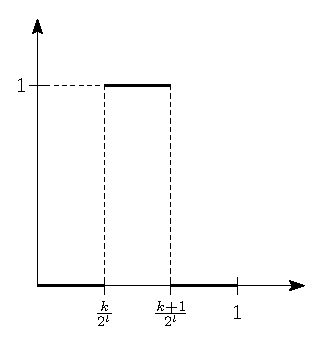
\includegraphics[width=0.3\textwidth]{RAL7_1.eps}
		\caption{Функция $\psi_{l,k}(x)$.}
		\label{7_1}
	\end{figure}
	Таким образом, ступенька пробегает весь отрезок $[0,1]$, затем её длина уменьшается вдвое и опять повторяется тоже самое. Тогда $\forall n \in \MN$ можно представить (однозначно) в виде: $n = 2^l + k$.
	При этом будет верно: $n \to \infty \Leftrightarrow l \to \infty$, поэтому:
	$$
		\forall n, \, \mu(\{x \in [0,1] \colon |f_n(x) - 0| > 0\}) = 2^{-l} \xrightarrow[n \to \infty]{} 0 \Rightarrow f_n \xRightarrow[ \lbrack 0,1 \rbrack ]{\mu} 0
	$$
	В тоже время $\forall x \in [0,1], \, \exists$ бесконечно много членов числовой последовательности $f_n(x) = 0$ и бесконечно много членов таких, что $f_n(x) = 1 \Rightarrow$ сходимости нет ни в одной точке.
\end{proof}

\begin{theorem}(\textbf{Рисса})
	Пусть $f_n \xRightarrow{\mu, X} f$, тогда существует подпоследовательность $\{f_{n_k}(x)\}_{k = 1}^{\infty}$ такая, что: 
	$$
		f_{n_k}(x) \xrightarrow{as, X} f(x)
	$$
\end{theorem}
\begin{proof}
	Пусть $\mu(X) < \infty$, тогда рассмотрим $n_i$ такие, что: 
	$$
		\mu(\{x \in X \colon |f_{n_i}(x) - f(x)| > 2^{-i}\}) < 2^{-i}
	$$
	где $i = 1,2, \dotsc$, также считаем, что $n_i$ монотонно возрастают. Проверим, что $f_{n_i}(x) \xrightarrow{as} f(x)$. Пусть заданы $\VE > 0$ и $\gamma > 0$, тогда если $i \colon 2^{-i} < \tfrac{1}{2}\min(\VE,\gamma)$, то:
	$$
		\mu\left(\bigcup\limits_{j = i}^{\infty}\{x \in X \colon |f_{n_j}(x) - f(x)| > \VE\}\right) \leq \mu\left(\bigcup\limits_{j = i}^{\infty}\{x \in X \colon |f_{n_j}(x) - f(x)| > 2^{-j}\}\right)
	$$
	поскольку множество справа более широкое, чем слева. Заметим, что:
	$$
		\mu\left(\bigcup\limits_{j = i}^{\infty}\{x \in X \colon |f_{n_j}(x) - f(x)| > 2^{-j}\}\right) \leq \ddsum{j = i}{\infty}\mu(\{x \in X \colon |f_{n_j}(x) - f(x)| > 2^{-j}\}) < \ddsum{j = i}{\infty}2^{-j} = 2^{i - 1}< \gamma
	$$
	Согласно критерию теоремы $3$, это означает, что: $f_{n_i}(x) \xrightarrow{as} f(x)$. Рассмотрим теперь другой случай: 
	$$
		X = \bigsqcup\limits_{k = 1}^{\infty}B_k, \; \forall k, \, \mu(B_k) < \infty 
	$$
	Поскольку из сходимости по мере на всём $X$ следует сходимость по мере на его подмножестве, то:
	$$
		f_n \xRightarrow{\mu} f \; \Rightarrow \; \forall k, \, f_n \xRightarrow{\mu, B_k} f
	$$ 
	Тогда, по доказанному выше существует последовательность $\{f_{1,n(1)}\}_{n(1) = 1}^{\infty}$, которая является подпоследовательностью: $F_0 = \{f_n\}_{n = 1}^{\infty}$ и при этом такая, что: 
	$$
		f_{1,n(1)} \xrightarrow{as, B_1} f
	$$ 
	Затем, поскольку: $f_{1,n(1)} \xRightarrow{\mu,B_2} f$, как часть последовательности, которая изначально сходилась по мере, то тогда: $\exists \, \{f_{2,n(2)}\}_{n(2) = 1}^{\infty}$, которая является подпоследовательностью последовательности: $\{f_{1,n(1)}\}_{n(1) = 1}^{\infty}$ и при этом такая, что: 
	$$
		f_{2,n(2)} \xrightarrow{as, B_2} f
	$$ 
	И так далее. Взяв диагональную последовательность: $\{f_{i,n(i)_i}(x)\}_{i = 1}^{\infty}$ мы получим, что она $\forall k$ сходится почти всюду на $B_k$. Если $A_k \subset B_k$ это множество, где сходимости нет, то: $\mu(A_k) = 0$. Следовательно: 
	$$
		\mu\left(\bigsqcup\limits_{k = 1}^{\infty}A_k\right) = 0
	$$ 
	На $X \setminus \bigsqcup\limits_{k = 1}^{\infty}A_k$ есть сходимость $\Rightarrow$ в случае $\sigma$-конечной меры, мы выделили сходящуюся почти всюду подпоследовательность.
\end{proof}

\begin{theorem}(\textbf{Егорова})
	Пусть $(X,\MM,\mu)$ - ИП, $\mu(X) < \infty$ и есть последовательность функций $\{f_n(x)\}_{n = 1}^{\infty}$ такая, что: $f_n(x) \xrightarrow{as} f(x)$. Тогда:
	$$
		\forall \VE > 0, \, \exists \, E_\VE \in \MM \colon \mu( E_\VE) < \VE, \quad \forall x \in X \setminus E_\VE, \,  f_n(x) \uconv{X \setminus E_\VE} f(x)
	$$
	То есть, принебрегая небольшой окрестностью из сходиомости п.в. следует равномерная сходимость.
\end{theorem}
\begin{proof}
	Согласно критерию теоремы $3$ будет верно:
	$$
		\forall i, \, \exists \, n_i \colon \mu\left(\bigcup\limits_{n = n_i}^{\infty}\{x \in X \colon |f_n(x) -f(x)| > \tfrac{1}{i}\}\right) < \dfrac{\VE}{2^{i+1}}, \, i  = 1,2,\dotsc
	$$
	Тогда: 
	$$
		E_\VE = \bigcup\limits_{i = 1}^{\infty}\bigcup\limits_{n = n_i}^{\infty}\{x \in X \colon |f_n(x) - f(x)| >\tfrac{1}{i}\} \Rightarrow \mu(E_\VE) \leq \ddsum{i = 1}{\infty}	\dfrac{\VE}{2^{i+1}} = \dfrac{\VE}{2} < \VE
	$$ 
	Пусть у нас задано $\gamma > 0 \Rightarrow \exists \, m \colon \tfrac{1}{m} < \gamma$. Заметим, что: 
	$$
		x \in X \setminus E_\VE \Rightarrow x \not\in \bigcup\limits_{n = n_m}^{\infty}\{x \in X \colon |f_n(x) - f(x)|> \tfrac{1}{m}\}
	$$ 
	Следовательно: 
	$$
		\forall n \geq n_m \Rightarrow |f_n(x) - f(x)| \leq \tfrac{1}{m} < \gamma
	$$ 
	А это и означает равномерную сходимость на $X \setminus E_\VE$.
\end{proof}


\textbf{Пример}: Если верно: 
$$
	f_n(x) = \chi_{(-n,n)}(x) = \MTI_{(-n,n)}(x)
$$ 
где $n = 1,2, \dotsc$, то тогда: $f_n(x) \xrightarrow{as} 1$ на $\MR^1$, но в то же время, нельзя выделить множество конечной меры на $\MR^1$ такое, что вне этого множества сходимость будет равномерной.

\begin{theorem}(\textbf{Лузин})
	Пусть $f(x)$ измерима на $[a,b] \subset \MR^1$ относительно классической меры Лебега и конечна почти всюду на $[a,b]$, тогда:
	$$
		\forall \VE > 0, \, \exists \, g_\VE(x) \in C([a,b]) \colon \mu(\{x \in [a,b] \colon f(x) \neq g(x)\}) < \VE
	$$	
\end{theorem}
\begin{rem}
	Теорема говорит о том, что если принебречь множеством сколь угодно малой меры, то можно из нашей произвольной, измеримой и конечной почти всюду функции сделать непрерывную функцию.
\end{rem}

\begin{rem}
	Теорема приводится без доказательства, ранее она доказывалась на семинарах.
\end{rem}

\end{document}